\begin{columns}[t]
	\begin{column}{0.50\textwidth}
		\begin{block}{\large Motivation for autonomous data generation}
		    	\begin{columns}[T]
		    		\centering
		    		\begin{column}{0.60\textwidth}
					    {\bf \quad Motivation:}
					    \begin{itemize}
						    \item State-of-the-art methods use Convolutional Neural Network (CNN) to perform object segmentation.
						    \item CNNs need access to a large set of labeled data, which requires intensive human labor.
						    \item Current techniques for generating synthetic dataset suffers from dataset bias as they lack realism.
					    \end{itemize}
					    \vspace{0.8in}
					    {\bf\quad Objective:}
					    \begin{itemize}
					    \item Generate a physically-realistic labeled dataset in an autonomous manner to train a CNN for object detection.
					    \end{itemize}
					\end{column}
					\begin{column}{0.40\textwidth}
						\centering
						\vspace{-0.2in}
						\begin{figure}[h]
							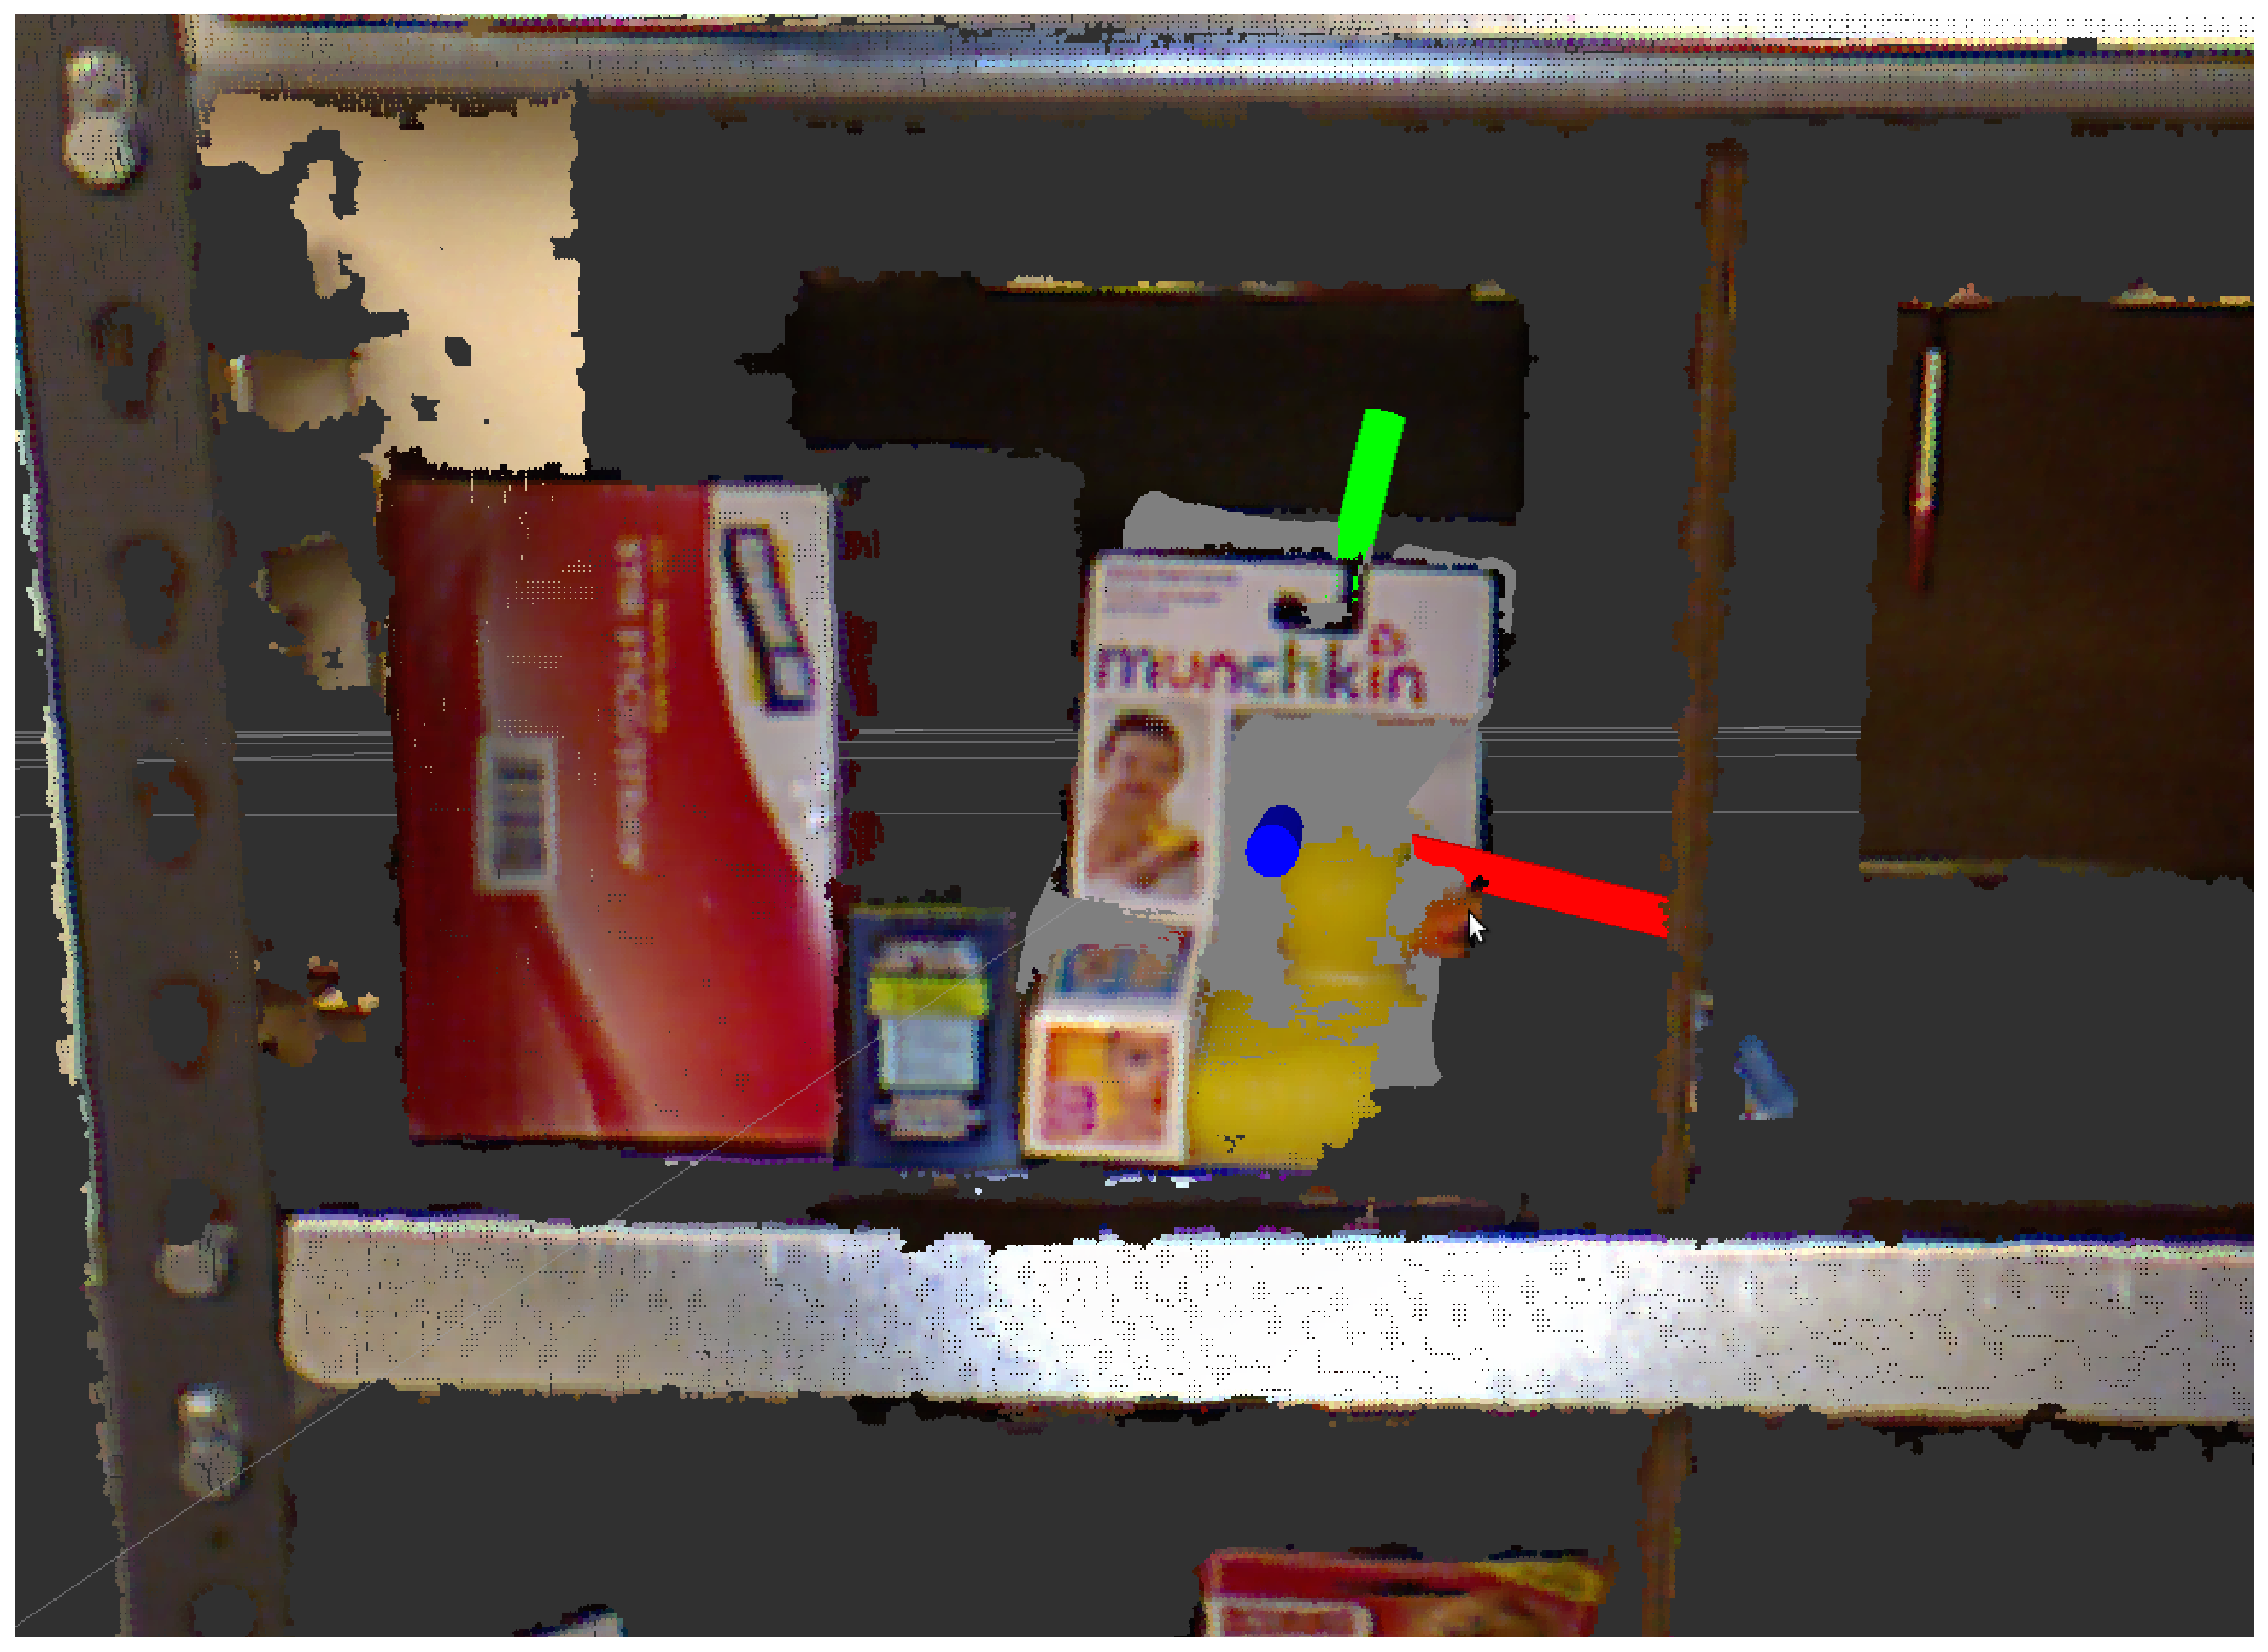
\includegraphics[width=0.75\textwidth]{manual_rutgers}
							\vspace{0.1in}
							\caption{Rutgers RGBD dataset with manual annotation}
						\end{figure}
						\vspace{0.3in}
						\begin{figure}[h]
							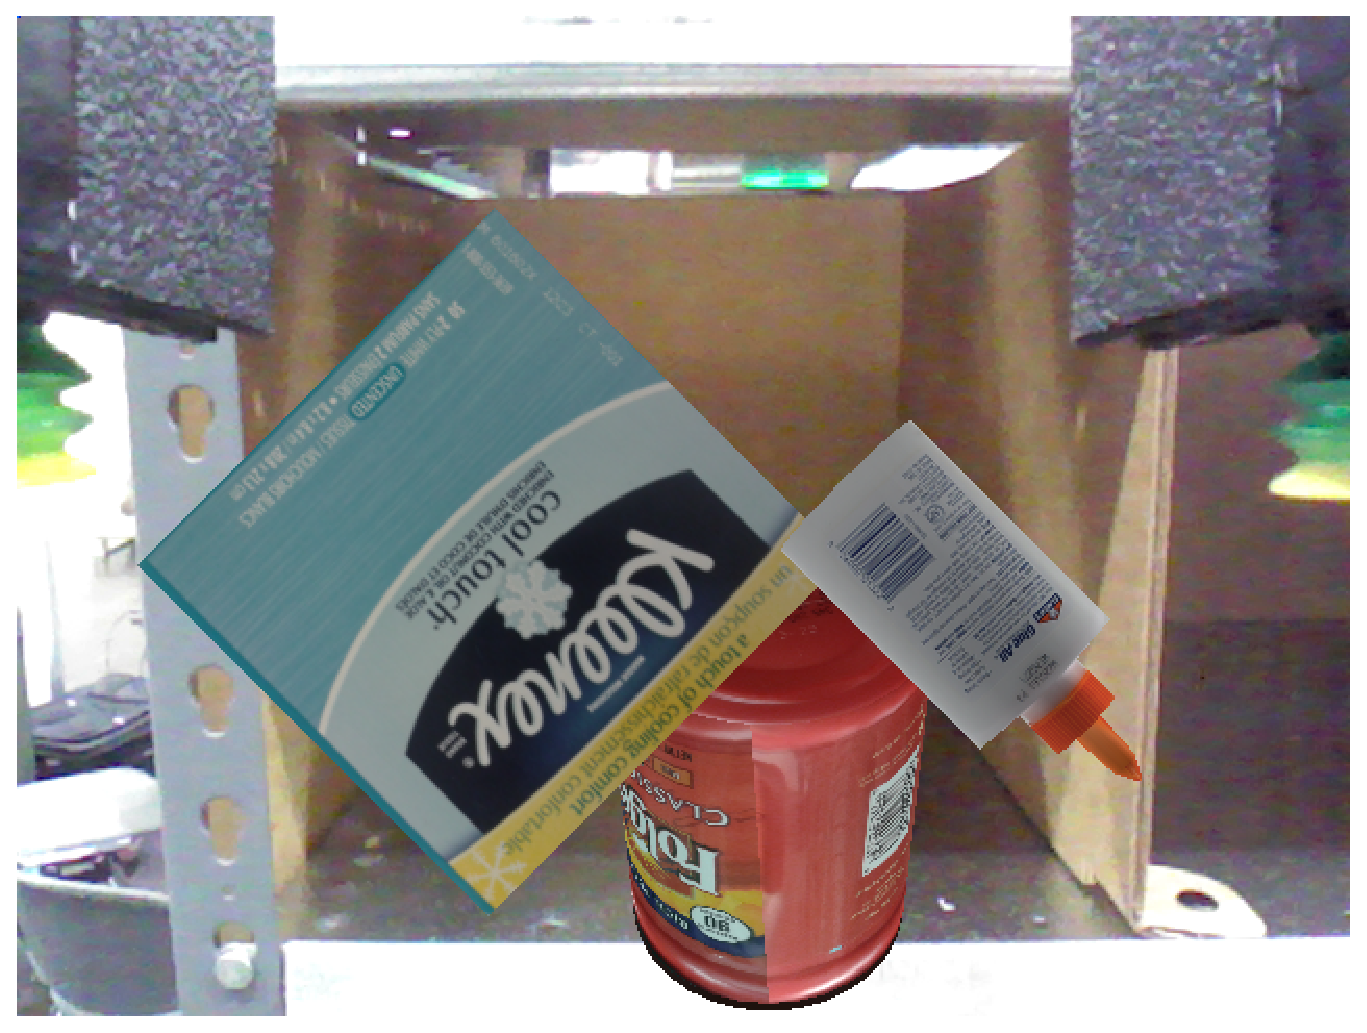
\includegraphics[width=0.75\textwidth]{unreal_syn}
							\vspace{0.1in}
							\caption{Physically unrealistic synthetic dataset generation}
						\end{figure}
					\end{column}
				\end{columns}
		\end{block}
	\end{column}
	\begin{column}{0.50\textwidth}
		\begin{block}{\large Using Physics Simulation to generate training dataset}
		\centering
		    \begin{itemize}
			    \item Environmental and geometric constraints are used to generate datasets for \\setups such as shelf bin and table-top.
			    \item Each scene is generated by randomly sampling object poses from a domain specified for the setup.
			    \item Physics simulation is performed for generating physically realistic scenes so that the training dataset captures appropriate object scales and occlusions.
		    \end{itemize}
		    \vspace{0.2in}
		    \begin{figure}[h]
				\includegraphics[width=0.80\textwidth]{physim}
				\caption{Pipeline for data generation using physics simulation}
			\end{figure}
		\end{block}
	\end{column}
\end{columns}	
		    
